\documentclass[11pt,a4paper]{article}

\usepackage[utf8]{inputenc}
\usepackage[T1]{fontenc}
\usepackage[spanish,es-nodecimaldot]{babel}
\usepackage{lmodern}
\usepackage{geometry}
\geometry{top=2.2cm,bottom=2.2cm,left=2.3cm,right=2.3cm}
\usepackage{graphicx}
\usepackage{booktabs}
\usepackage{tabularx}
\usepackage{array}
\usepackage{float}
\usepackage{caption}
\usepackage{xcolor}
\usepackage{fancyhdr}
\usepackage{enumitem}
\usepackage{hyperref}
\usepackage{microtype}
\usepackage{titlesec}
\usepackage{siunitx}

\definecolor{azulproyecto}{HTML}{175B8F}
\definecolor{azulclaro}{HTML}{EAF3F8}
\definecolor{gristexto}{HTML}{424B54}
\definecolor{grisfila}{HTML}{F4F6F7}

\hypersetup{
    colorlinks=true,
    linkcolor=azulproyecto,
    urlcolor=azulproyecto,
    pdftitle={Diseño de caja electrónica, esquemático y PCB - VehicleSense},
    pdfauthor={Patricio Vásquez}
}

\pagestyle{fancy}
\fancyhf{}
\lhead{VehicleSense}
\rhead{Diseño de caja y PCB}
\cfoot{\thepage}
\renewcommand{\headrulewidth}{0.4pt}
\setlength{\headheight}{14pt}

\titleformat{\section}
  {\Large\bfseries\color{azulproyecto}}
  {\thesection.}{0.6em}{}
\titleformat{\subsection}
  {\large\bfseries\color{gristexto}}
  {\thesubsection.}{0.5em}{}

\captionsetup{
    font=small,
    labelfont=bf,
    justification=centering
}

\setlist[itemize]{leftmargin=1.4em,itemsep=0.25em,topsep=0.35em}
\setlist[enumerate]{leftmargin=1.6em,itemsep=0.35em,topsep=0.35em}
\renewcommand{\arraystretch}{1.25}

\newcommand{\dato}[1]{\textbf{#1}}

\begin{document}

% -----------------------------------------------------------------------------
% PORTADA
% -----------------------------------------------------------------------------
\begin{titlepage}
    \thispagestyle{empty}
    \color{black}
    \begin{flushright}
        
\includegraphics[width=5.4cm]{../recursos/espol_logo.png}
    \end{flushright}
    \vspace{1.15cm}
    \begin{center}
        {\Large\bfseries ESCUELA SUPERIOR POLITÉCNICA DEL LITORAL\par}
        \vspace{2.15cm}
        {\Large\bfseries FACULTAD DE INGENIERÍA EN MECÁNICA\\
        Y CIENCIAS DE LA PRODUCCIÓN\par}
        \vspace{1.75cm}
        {\Large\bfseries ITINERARIO DE INVESTIGACIÓN\par}
        \vspace{1.55cm}
        {\Large\bfseries INFORME TÉCNICO IV\par}
        \vspace{0.6cm}
        {\LARGE\bfseries DISEÑO DE LA CAJA ELECTRÓNICA, ESQUEMÁTICO Y PCB\par}
        \vspace{0.5cm}
        {\large Dispositivo de monitoreo multisensorial para vehículos\par}
        \vfill
        {\large\bfseries Autor\par}
        \vspace{0.45cm}
        {\Large\bfseries Vásquez Villarreal Patricio Andrés\par}
        \vspace{1.25cm}
        {\large\bfseries Término académico\par}
        \vspace{0.45cm}
        {\Large\bfseries 2026 PAO 1\par}
    \end{center}
    \vspace{0.6cm}
\end{titlepage}

\tableofcontents
\clearpage

% -----------------------------------------------------------------------------
\section{Introducción}

VehicleSense es un dispositivo electrónico de monitoreo multisensorial destinado a
vehículos. Su función es integrar en una sola unidad el microcontrolador, los sensores,
el sistema de posicionamiento, el almacenamiento local y los elementos de comunicación.
Para convertir el prototipo en un conjunto físico ordenado y transportable se diseñaron
tres elementos principales:

\begin{itemize}
    \item una caja electrónica fabricable mediante impresión 3D;
    \item un esquemático que define las conexiones entre el ESP32 y los módulos;
    \item una tarjeta PCB que organiza físicamente los conectores, la alimentación y el cableado.
\end{itemize}

El presente documento describe estos elementos de forma resumida, con énfasis en las
medidas implementadas, la distribución de componentes y las consideraciones necesarias
para el ensamblaje del prototipo.

\paragraph{Repositorio del proyecto.}
El código fuente y los recursos técnicos de VehicleSense se encuentran disponibles en
\href{https://github.com/PatricioV1207/Multisensory-Device}{github.com/PatricioV1207/Multisensory-Device}.

\section{Objetivo del diseño}

El objetivo del diseño mecánico y electrónico es disponer de un módulo compacto que
permita instalar el sistema de monitoreo dentro de un vehículo sin depender de una gran
cantidad de cables sueltos. La caja protege la electrónica y proporciona accesos para
conectores, mientras que la PCB centraliza las conexiones de los sensores y reduce el
riesgo de errores durante el montaje.

Los criterios principales considerados fueron:

\begin{itemize}
    \item espacio suficiente para la PCB y sus módulos;
    \item fijación mediante tornillos y separadores;
    \item aberturas para cableado y acceso a componentes;
    \item posibilidad de retirar la tapa para mantenimiento;
    \item distribución de conectores cercana a los bordes de la PCB;
    \item filtrado de alimentación y tierra común entre los módulos.
\end{itemize}

% -----------------------------------------------------------------------------
\section{Diseño de la caja electrónica}

La envolvente fue modelada de forma paramétrica en OpenSCAD. Está compuesta por una
base y una tapa independientes, ambas con esquinas redondeadas y cuatro puntos de cierre.
El tamaño exterior seleccionado es de \SI{115}{\milli\metre} por \SI{95}{\milli\metre},
lo que proporciona una superficie suficiente para alojar la tarjeta y permitir el paso
de conductores hacia los conectores laterales.

\subsection{Dimensiones principales}

\begin{table}[H]
\centering
\caption{Dimensiones generales implementadas en la caja.}
\begin{tabularx}{0.96\textwidth}{>{\bfseries}p{5.4cm} X >{\raggedleft\arraybackslash}p{3.0cm}}
\toprule
Parámetro & Descripción & Valor \\
\midrule
Largo exterior & Dimensión principal de la envolvente en el eje X & \SI{115}{\milli\metre} \\
Ancho exterior & Dimensión principal de la envolvente en el eje Y & \SI{95}{\milli\metre} \\
Altura interior útil & Espacio vertical disponible dentro de la base & \SI{22}{\milli\metre} \\
Espesor de base y tapa & Espesor nominal de las superficies horizontales & \SI{1.6}{\milli\metre} \\
Altura del cuerpo sin tapa & Altura interior más el espesor del fondo & \SI{23.6}{\milli\metre} \\
Espesor de pared & Grosor de las paredes laterales & \SI{3.6}{\milli\metre} \\
Radio de las esquinas & Redondeo exterior de las cuatro esquinas & \SI{6}{\milli\metre} \\
Diámetro de cierre & Perforaciones de las cuatro esquinas & \SI{3.2}{\milli\metre} \\
Altura del reborde de acople & Guía utilizada para alinear base y tapa & \SI{2}{\milli\metre} \\
Tolerancia del acople & Holgura prevista para compensar la impresión 3D & \SI{0.8}{\milli\metre} \\
\bottomrule
\end{tabularx}
\end{table}

Considerando el espesor de las paredes, el área interior rectangular teórica es de
aproximadamente \SI{107.8}{\milli\metre} por \SI{87.8}{\milli\metre}. En las esquinas
esta área se reduce por el redondeo y por los postes de cierre, por lo que la tarjeta
debe verificarse con el modelo físico antes de realizar la instalación definitiva.

\subsection{Aberturas implementadas}

La caja incorpora tres aberturas destinadas al acceso de cables, conectores o elementos
que deban quedar expuestos. Sus dimensiones son las siguientes:

\begin{table}[H]
\centering
\caption{Aberturas realizadas en la envolvente.}
\begin{tabularx}{0.96\textwidth}{>{\bfseries}p{3.4cm} p{3.7cm} X}
\toprule
Ubicación & Dimensiones & Posición implementada \\
\midrule
Lateral frontal & Óvalo horizontal de \SI{13.3}{\milli\metre} por \SI{5.4}{\milli\metre} & Centrado en el largo de la caja y a \SI{12.6}{\milli\metre} desde la cara inferior. \\
Lateral posterior & Orificio circular de \SI{7.6}{\milli\metre} de diámetro & Centrado en el largo de la caja y a la misma altura que la abertura ovalada. \\
Tapa & Rectángulo de \SI{15}{\milli\metre} por \SI{25}{\milli\metre} & Centro situado en $x=\SI{32.5}{\milli\metre}$ y $y=\SI{67.5}{\milli\metre}$, medidos desde una esquina de referencia. \\
\bottomrule
\end{tabularx}
\end{table}

La abertura rectangular se encuentra desplazada \SI{25}{\milli\metre} hacia la izquierda
y \SI{20}{\milli\metre} hacia la parte superior con respecto al centro geométrico de la
tapa. Esta posición evita la zona central de la PCB y mantiene un margen alrededor del
perímetro.

\subsection{Fijación de la PCB}

La base incluye cuatro perforaciones para tornillos M3 y anillos de refuerzo internos.
Estos puntos permiten sujetar separadores metálicos o de nylon desde la parte inferior.
La cabeza del tornillo puede quedar embutida para mantener la superficie exterior lo más
plana posible.

\begin{table}[H]
\centering
\caption{Características de los puntos de montaje de la PCB.}
\begin{tabularx}{0.96\textwidth}{>{\bfseries}p{5.3cm} X >{\raggedleft\arraybackslash}p{3.1cm}}
\toprule
Parámetro & Función & Valor \\
\midrule
Separación horizontal & Distancia entre centros de fijación en X & \SI{85}{\milli\metre} \\
Separación vertical & Distancia entre centros de fijación en Y & \SI{65}{\milli\metre} \\
Diámetro pasante & Holgura para tornillo M3 & \SI{3.4}{\milli\metre} \\
Diámetro del avellanado & Alojamiento inferior de la cabeza & \SI{6.5}{\milli\metre} \\
Profundidad del avellanado & Coincide con el espesor del fondo & \SI{1.6}{\milli\metre} \\
Diámetro del refuerzo interno & Superficie de apoyo del separador & \SI{9}{\milli\metre} \\
Altura del refuerzo interno & Elevación adicional sobre el fondo & \SI{2.5}{\milli\metre} \\
\bottomrule
\end{tabularx}
\end{table}

Tomando como origen una esquina de la caja, los centros de los cuatro puntos de montaje
se ubican aproximadamente en $(15,15)$, $(100,15)$, $(15,80)$ y $(100,80)$ mm.

\clearpage
\begin{figure}[H]
    \centering
    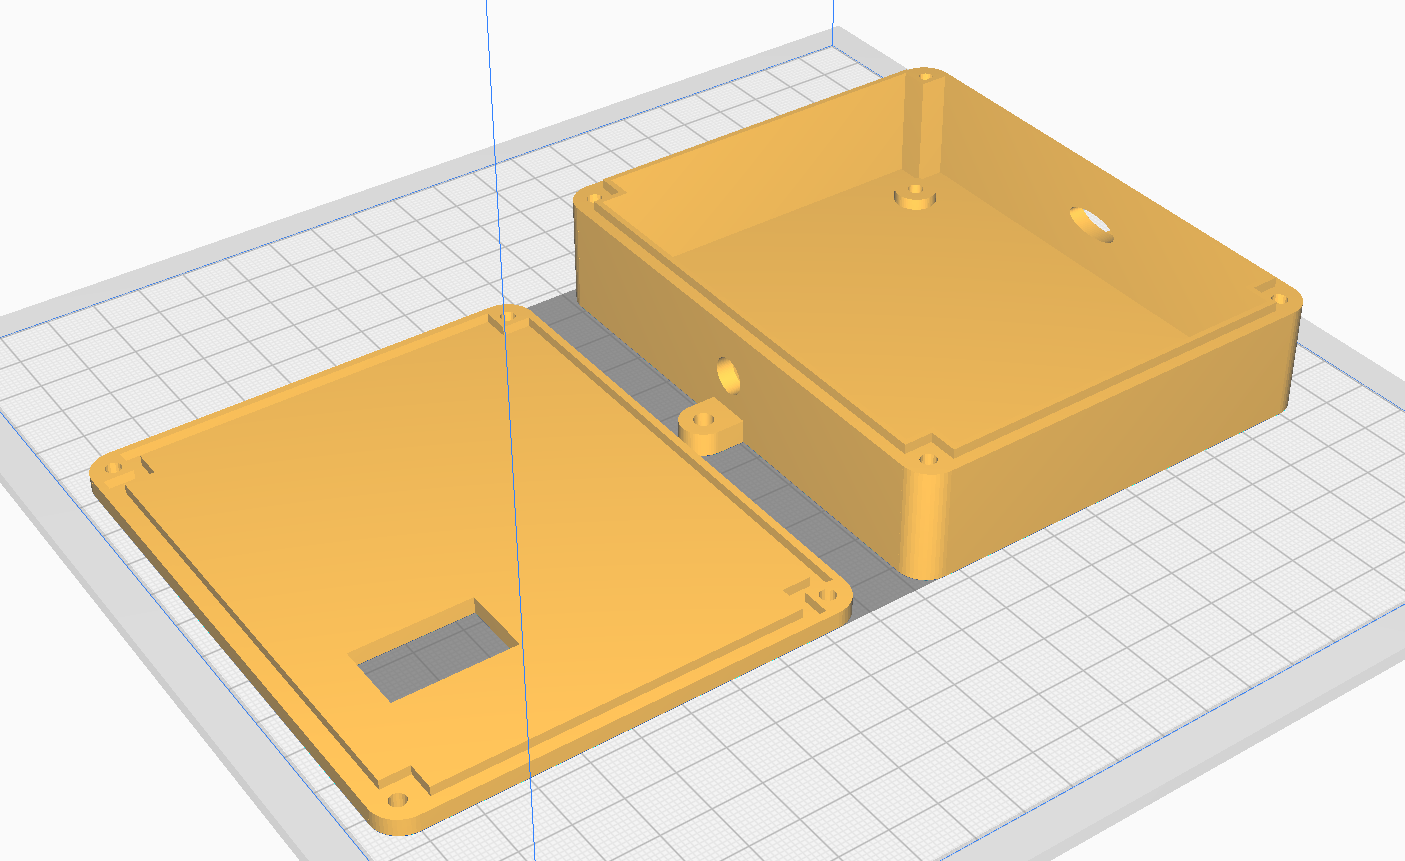
\includegraphics[width=0.98\textwidth]{imagenes/caja_3d.png}
    \caption{Vista tridimensional de la base y la tapa de la caja electrónica.}
    \label{fig:caja3d}
\end{figure}

En la Figura~\ref{fig:caja3d} se observan el reborde de acople, las cuatro perforaciones
de cierre, los puntos interiores de fijación, las dos aberturas laterales y el recorte
rectangular de la tapa. La geometría permite imprimir las dos piezas por separado y
ensamblarlas después de instalar la electrónica.

% -----------------------------------------------------------------------------
\section{Esquemático de conexiones}

El esquemático concentra las conexiones del sistema alrededor del ESP32-WROOM-32. El
microcontrolador funciona como unidad de adquisición y procesamiento, mientras que los
módulos externos se conectan mediante UART, I2C, SPI, I2S y entradas digitales.

\begin{figure}[H]
    \centering
    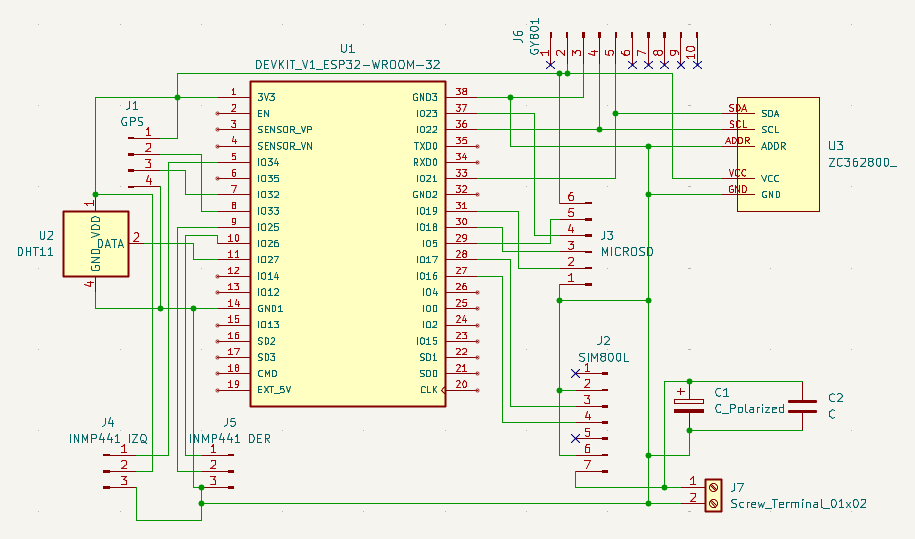
\includegraphics[width=0.99\textwidth]{imagenes/esquematico.png}
    \caption{Esquemático general de conexiones del prototipo.}
    \label{fig:esquematico}
\end{figure}

\subsection{Bloques representados}

El esquema mostrado en la Figura~\ref{fig:esquematico} incluye:

\begin{itemize}
    \item placa ESP32 DevKit como controlador principal;
    \item conector para el receptor GPS;
    \item sensor DHT11 para temperatura y humedad;
    \item cabecera del conjunto inercial GY-801;
    \item módulo de iluminación conectado al bus I2C;
    \item conector para módulo microSD;
    \item conector para el módem SIM800L;
    \item dos cabeceras previstas para micrófonos INMP441 izquierdo y derecho;
    \item bornera de alimentación y capacitores de filtrado.
\end{itemize}

\subsection{Interfaces y pines principales}

\begin{table}[H]
\centering
\caption{Resumen funcional de las conexiones principales.}
\begin{tabularx}{0.98\textwidth}{>{\bfseries}p{3.0cm} p{3.0cm} p{3.0cm} X}
\toprule
Módulo & Interfaz & Pines ESP32 & Función \\
\midrule
DHT11 & Digital & GPIO27 & Medición de temperatura y humedad. \\
GPS NEO-6M & UART2 & GPIO32 / GPIO33 & Recepción de sentencias NMEA y configuración opcional. \\
GY-801 & I2C & GPIO21 / GPIO22 & Acelerómetro, giroscopio, magnetómetro y barómetro. \\
Sensor de luz & I2C & GPIO21 / GPIO22 & Medición de iluminancia mediante el bus compartido. \\
MicroSD & SPI & GPIO18, 19, 23 y 5 & Registro local de telemetría y datos de diagnóstico. \\
SIM800L & UART1 & GPIO16 / GPIO17 & Comunicación celular prevista como expansión. \\
INMP441 & I2S & GPIO25, 26 y entrada de datos & Captura acústica digital; la configuración final debe validarse con el firmware utilizado. \\
\bottomrule
\end{tabularx}
\end{table}

Los módulos I2C comparten las líneas SDA y SCL, por lo que cada dispositivo debe mantener
una dirección diferente. La microSD utiliza un bus SPI independiente y el GPS emplea un
puerto UART dedicado. Esta separación reduce interferencias entre periféricos y facilita
las pruebas individuales.

\subsection{Alimentación y filtrado}

La entrada de energía se realiza mediante la bornera J7. Los capacitores C1 y C2 se
encargan de reducir variaciones y ruido sobre la alimentación. El capacitor electrolítico
proporciona reserva de energía ante cambios de carga, mientras que el capacitor de menor
valor ayuda a filtrar componentes de mayor frecuencia.

El SIM800L no debe alimentarse directamente desde la salida de \SI{3.3}{\volt} del ESP32.
Cuando se incorpore la comunicación celular debe utilizarse una fuente capaz de soportar
picos de corriente elevados, con tierra común y un capacitor cercano al módem. El sistema
puede operar inicialmente mediante WiFi conservando el conector celular para una fase
posterior.

% -----------------------------------------------------------------------------
\section{Diagrama de la PCB}

La PCB transforma el esquemático en una distribución física. El ESP32 se ubica en la
zona central y los conectores se sitúan alrededor de sus bordes para facilitar el acceso
a los módulos y reducir el cruce de conductores.

\begin{figure}[H]
    \centering
    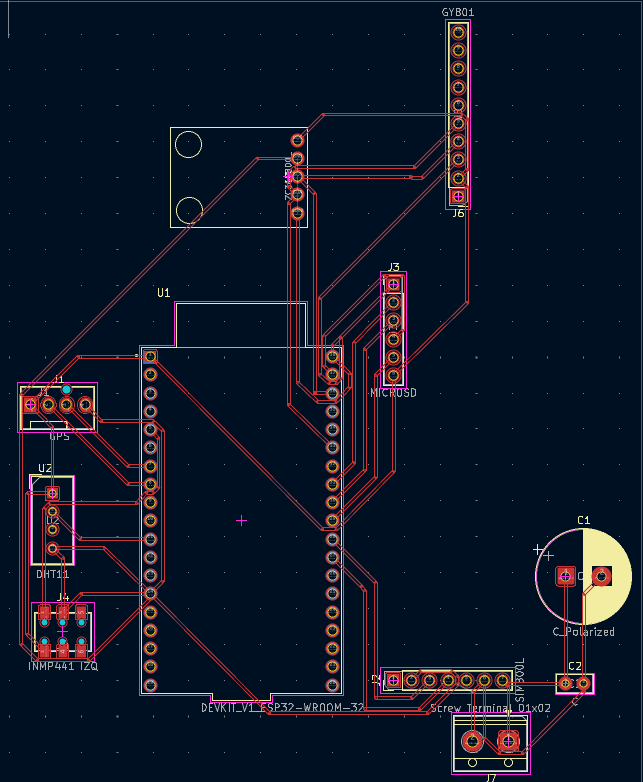
\includegraphics[height=0.76\textheight]{imagenes/pcb_layout.png}
    \caption{Distribución y enrutamiento de la tarjeta PCB.}
    \label{fig:pcblayout}
\end{figure}

\subsection{Distribución de componentes}

En la Figura~\ref{fig:pcblayout} se aprecia la siguiente organización:

\begin{itemize}
    \item el footprint principal del ESP32 ocupa la zona central;
    \item los sensores de ambiente y las cabeceras de micrófono están próximos a un borde;
    \item el conector del GY-801 se encuentra en la parte superior;
    \item la microSD y el SIM800L poseen cabeceras independientes;
    \item la bornera y los capacitores están agrupados en la zona de alimentación;
    \item las pistas se dirigen desde el controlador hacia cada conector siguiendo recorridos directos.
\end{itemize}

Esta distribución permite retirar o sustituir módulos sin desoldar el microcontrolador.
Además, ubicar los conectores cerca del perímetro facilita que los cables coincidan con
las aberturas de la caja.

\subsection{Consideraciones del trazado}

Para la fabricación definitiva deben verificarse los siguientes aspectos:

\begin{itemize}
    \item aumentar el ancho de las pistas que transportan alimentación;
    \item mantener una referencia de tierra continua y de baja impedancia;
    \item separar las líneas del micrófono I2S de la alimentación pulsante del módem;
    \item evitar pistas largas alrededor de las señales SPI de la microSD;
    \item comprobar que los conectores no interfieran con la tapa ni con los separadores;
    \item incluir los cuatro orificios de montaje de acuerdo con el patrón de \SI{85}{\milli\metre} por \SI{65}{\milli\metre}.
\end{itemize}

La captura representa el estado actual del trazado. Antes de ordenar la placa se debe
ejecutar la revisión de reglas eléctricas y de diseño, además de comprobar la orientación
de cada conector con los módulos físicos.

% -----------------------------------------------------------------------------
\section{Vista tridimensional de la PCB}

La vista 3D permite revisar la distribución mecánica, la orientación de conectores y la
altura aproximada de algunos componentes antes de fabricar la tarjeta.

\begin{figure}[H]
    \centering
    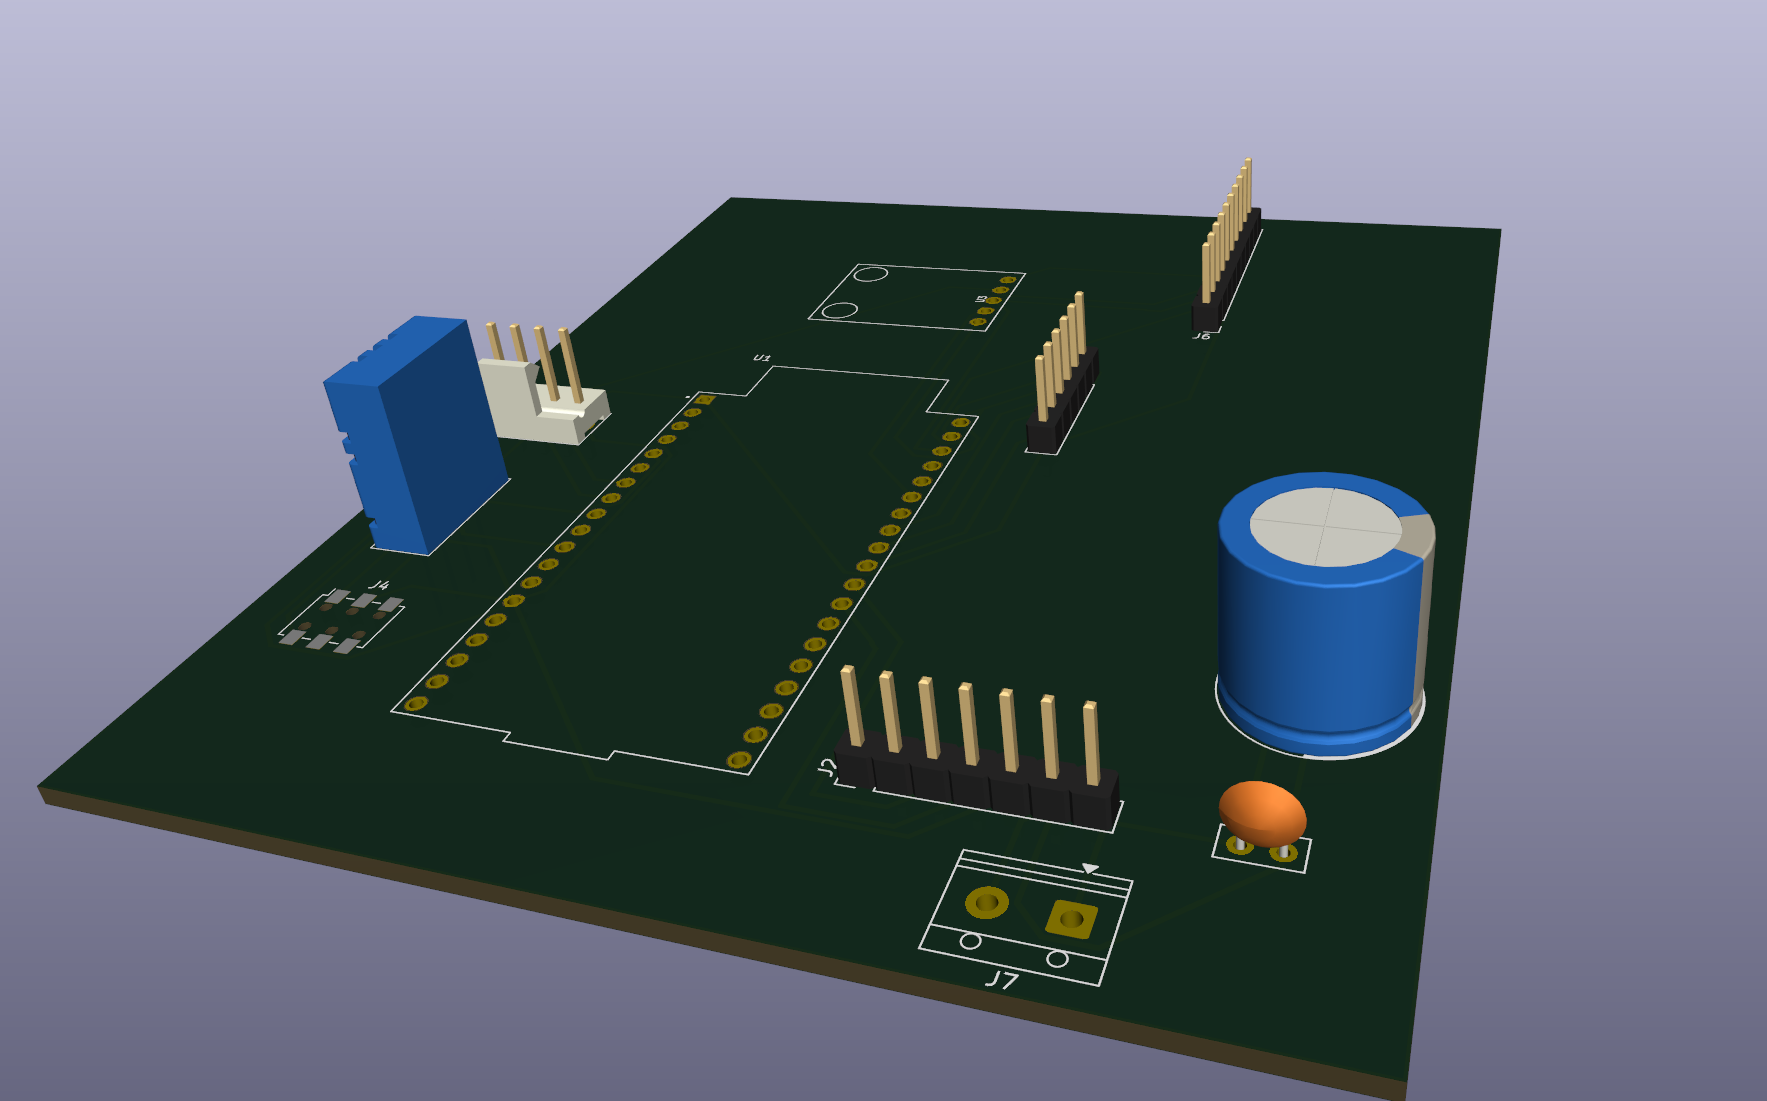
\includegraphics[width=0.98\textwidth]{imagenes/pcb_3d.png}
    \caption{Vista tridimensional de la tarjeta PCB.}
    \label{fig:pcb3d}
\end{figure}

En la Figura~\ref{fig:pcb3d} se distinguen la bornera, el sensor DHT11, los capacitores y
varias cabeceras. Algunos módulos aparecen únicamente como contornos o footprints porque
sus modelos tridimensionales todavía no están asignados. Esto no afecta la conectividad
del esquemático, pero limita la verificación de alturas y posibles colisiones.

Antes del ensamblaje final se recomienda agregar o comprobar los modelos 3D del ESP32,
la microSD, el SIM800L, el GPS y el GY-801. La altura total de estos módulos debe ser menor
que la altura interior disponible de \SI{22}{\milli\metre}, considerando también el
separador, el espesor de la PCB, las soldaduras y los conectores.

% -----------------------------------------------------------------------------
\section{Integración de la PCB con la caja}

La integración mecánica se realiza colocando cuatro separadores sobre los refuerzos de
la base. La PCB se fija a estos separadores y los tornillos se introducen desde la parte
inferior, utilizando el avellanado para evitar que las cabezas sobresalgan.

El procedimiento de montaje recomendado es:

\begin{enumerate}
    \item imprimir la base y la tapa y retirar soportes o rebabas;
    \item verificar los diámetros de las perforaciones con tornillos M3;
    \item instalar los cuatro separadores sobre la base;
    \item colocar la PCB sin componentes altos y comprobar el patrón de montaje;
    \item ensamblar los módulos y revisar que los conectores queden orientados hacia las aberturas;
    \item conectar la alimentación y realizar una prueba funcional con la tapa abierta;
    \item cerrar la caja y comprobar que no exista presión sobre cables, antenas o sensores.
\end{enumerate}

La abertura ovalada puede utilizarse para un cable plano o conector de poca altura. El
orificio circular es apropiado para un cable individual, prensaestopa pequeño o acceso
a un conector. La función definitiva de cada abertura debe definirse con los componentes
físicos colocados, evitando doblar excesivamente los conductores.

\section{Recomendaciones de fabricación}

Para un primer prototipo se puede utilizar PLA, debido a su facilidad de impresión. Sin
embargo, para una instalación prolongada dentro de un vehículo es preferible evaluar PETG
o un material con mejor resistencia térmica. La temperatura interna de un vehículo cerrado
puede deformar materiales con baja tolerancia al calor.

Como configuración inicial de impresión se recomienda:

\begin{itemize}
    \item altura de capa de aproximadamente \SI{0.20}{\milli\metre};
    \item cuatro perímetros para mejorar la rigidez de paredes y postes;
    \item relleno entre 25\% y 35\%;
    \item orientación con el fondo de la base apoyado sobre la cama;
    \item impresión de la tapa con su cara exterior apoyada, siempre que el acabado requerido lo permita;
    \item prueba previa de tolerancia del reborde antes de imprimir la pieza completa.
\end{itemize}

También se debe comprobar que los orificios avellanados no reduzcan excesivamente el
espesor resistente del fondo. Si la cabeza del tornillo no queda completamente embutida,
puede corregirse el diámetro o utilizar tornillería de cabeza más pequeña.

\section{Conclusiones}

El diseño desarrollado integra la parte mecánica y electrónica del dispositivo
VehicleSense en un conjunto compacto. La caja de \SI{115}{\milli\metre} por
\SI{95}{\milli\metre} proporciona espacio para la PCB, incluye puntos de fijación M3,
aberturas laterales y una tapa desmontable. El patrón de montaje de
\SI{85}{\milli\metre} por \SI{65}{\milli\metre} permite sujetar la tarjeta mediante
separadores y tornillos avellanados.

El esquemático reúne las interfaces del ESP32 con los sensores, el GPS, la microSD, los
micrófonos y el conector celular. La PCB organiza estas conexiones y aproxima los
conectores a los bordes para facilitar la integración dentro de la envolvente. La vista
tridimensional permite revisar el montaje, aunque todavía es necesario completar algunos
modelos 3D y validar las alturas con los componentes reales.

Antes de fabricar la versión definitiva se recomienda realizar una impresión de prueba,
verificar físicamente el ajuste de la PCB, ejecutar las revisiones eléctricas del diseño
y confirmar que todas las conexiones coincidan con el firmware. Con estas validaciones,
el conjunto puede utilizarse como base mecánica y electrónica del prototipo multisensorial
para vehículos.

\end{document}
